\chapter{Jet Results and Discussion} \label{ch:analysis}

Beginning in March of 2012, the LHC began seven months of pp collisions at $\sqrt{s} = \,$ 8 TeV.  The jet cross sections and ratios of the cross sections for jets of different radii offers a unique perspective on the pQCD effects of hadronization at this new energy frontier.  Due to the expectation that no QGP is formed in a pp collision these measurements serve as a baseline for separating phenomena associated with the QGP in heavy-ion collisions.  In order to measure the jet cross section the following formula is used,

\begin{equation}
	\frac{d^{2} \sigma^{jet}}{d\eta \, dp_{T}} = \frac{A_{trigger}}{\epsilon_{trigger}(p_{T})} \times C_{MC} \times \frac{1}{A(p_{T}) } \times \frac{1}{\mathscr{L}_{int}} \times \frac{dN^{jet}}{dp_{T} \, d\eta}
\label{eq:xsecdef}
\end{equation}

\noindent
where,

\begin{itemize}
  \item $A_{trigger}$ is the acceptance for EMCal triggered events and $\epsilon_{trigger}(p_{T})$ is the EMCal trigger efficiency.  These factors correct for imperfections in the electronics of the EMCal and the overall factors are equal to one in minimum bias events.
  \item $C_{MC}$ is a correction factor due to detector effects and it allows for comparisons between the ALICE experiment to other experiments or theoretical calculations.  Unfolding is used to determine this factor.
  \item $\mathscr{L}_{int}$ is the integrated luminosity during the period when the data was recorded.
  \item $A(p_{T})$ is the geometrical detector acceptance.
  \item $\frac{dN^{jet}}{dp_{T} \, d\eta}$ is the inclusive jet momentum spectra.
  
\end{itemize}

\noindent
Furthermore, it is useful to define the ratio of cross sections,

\begin{equation}
\mathscr{R}(p_{T};R_{1},R_{2}) = \frac{d^{2}\sigma(p_{T};R_{1})/d\eta \, dp_{T}}{d^{2}\sigma(p_{T};R_{2})/d\eta \, dp_{T}}
\label{eq:xsecratio}
\end{equation}

\noindent
where $\sigma(p_{T};R_{1})$ refers to the doubly differential cross section (Equation \ref{eq:xsecdef}) of a jet with radius $R_{1}$.  The ratio is carried out on a bin--by--bin basis per each $p_{T}$ bin.  

\section{Raw Jet Spectra}

This thesis reports inclusive jet results for radii between 0.1 and 0.5.  Furthermore, jet results for radii R = 0.2 and R = 0.4 will be presented in the body of this chapter while results from the other radii will be limited to the appendix.  Figure shows the raw (uncorrected) $p_{T}$ spectra for inclusive jets from both MB and EMCal triggered data.  It is also evident from Figure that the Emcla triggered data extends the $p_{T}$ reach 



\section{8 TeV Data Quality}
ALICE is a state-of-the-art experiment with excellent tracking and particle identification capabilities as discussed in Chapter \ref{ch:alice}.  However, just like any real world experiment, it contains a number of inefficiencies and imperfections.  This means that the data collected during the 8 TeV pp collision must be examined and any inaccuracies in the data must be removed before hard physics conclusions may be reached.  Data may be compromised at both the event-level, the experiment erroneously recorded something as an event, or at the constituent-level, one of the subdetectors mismeasured a feature of a particle, and these outliers must be accounted for and removed 

\section{Event Selection}

For an event to be selected into a physics analysis it must pass a number of quality control tests.  For example, the LHC must have be in a state of stable beams, cosmic rays must be excluded by only accepting tracks that originate from a vertex inside the detector, and the relevant detectors for a given analysis must be functioning as intended.  Event selction and QA is implemented via a centralized class, AliEventCuts, within the AliRoot framework.  This class contains a number of corrections including:

\begin{itemize}
  \item 
  \item Another entry in the list
\end{itemize}

Further more the class AliAnalysisTaskEmcalCorrection within the AliRoot framework performs a number of corrections to the tower-level within phyasics analysis dependent on the EMCal.  These corrections include:

\begin{itemize}
  \item Energy calibration:  Remove double counting due to the amount of energy typically deposited by a Hadron.
  \item Bad Channel Map: Remove both dead and hot towers from the EMCal clusterize based on an iterative average energy per occupancy algoritham
  \item Time Calibration:  Remove slow particles, such as neutrons, which readout to the EMCal after the event has been recorded.
   \item Exotics Correction:  Remove inefficiencies due to how a particle interacted with the EMCal.
\end{itemize}\

After the above cuts are performed on EMCal towers the cells compromising the towers are clustered together using a clusterization algoritham 



\begin{figure}[h]
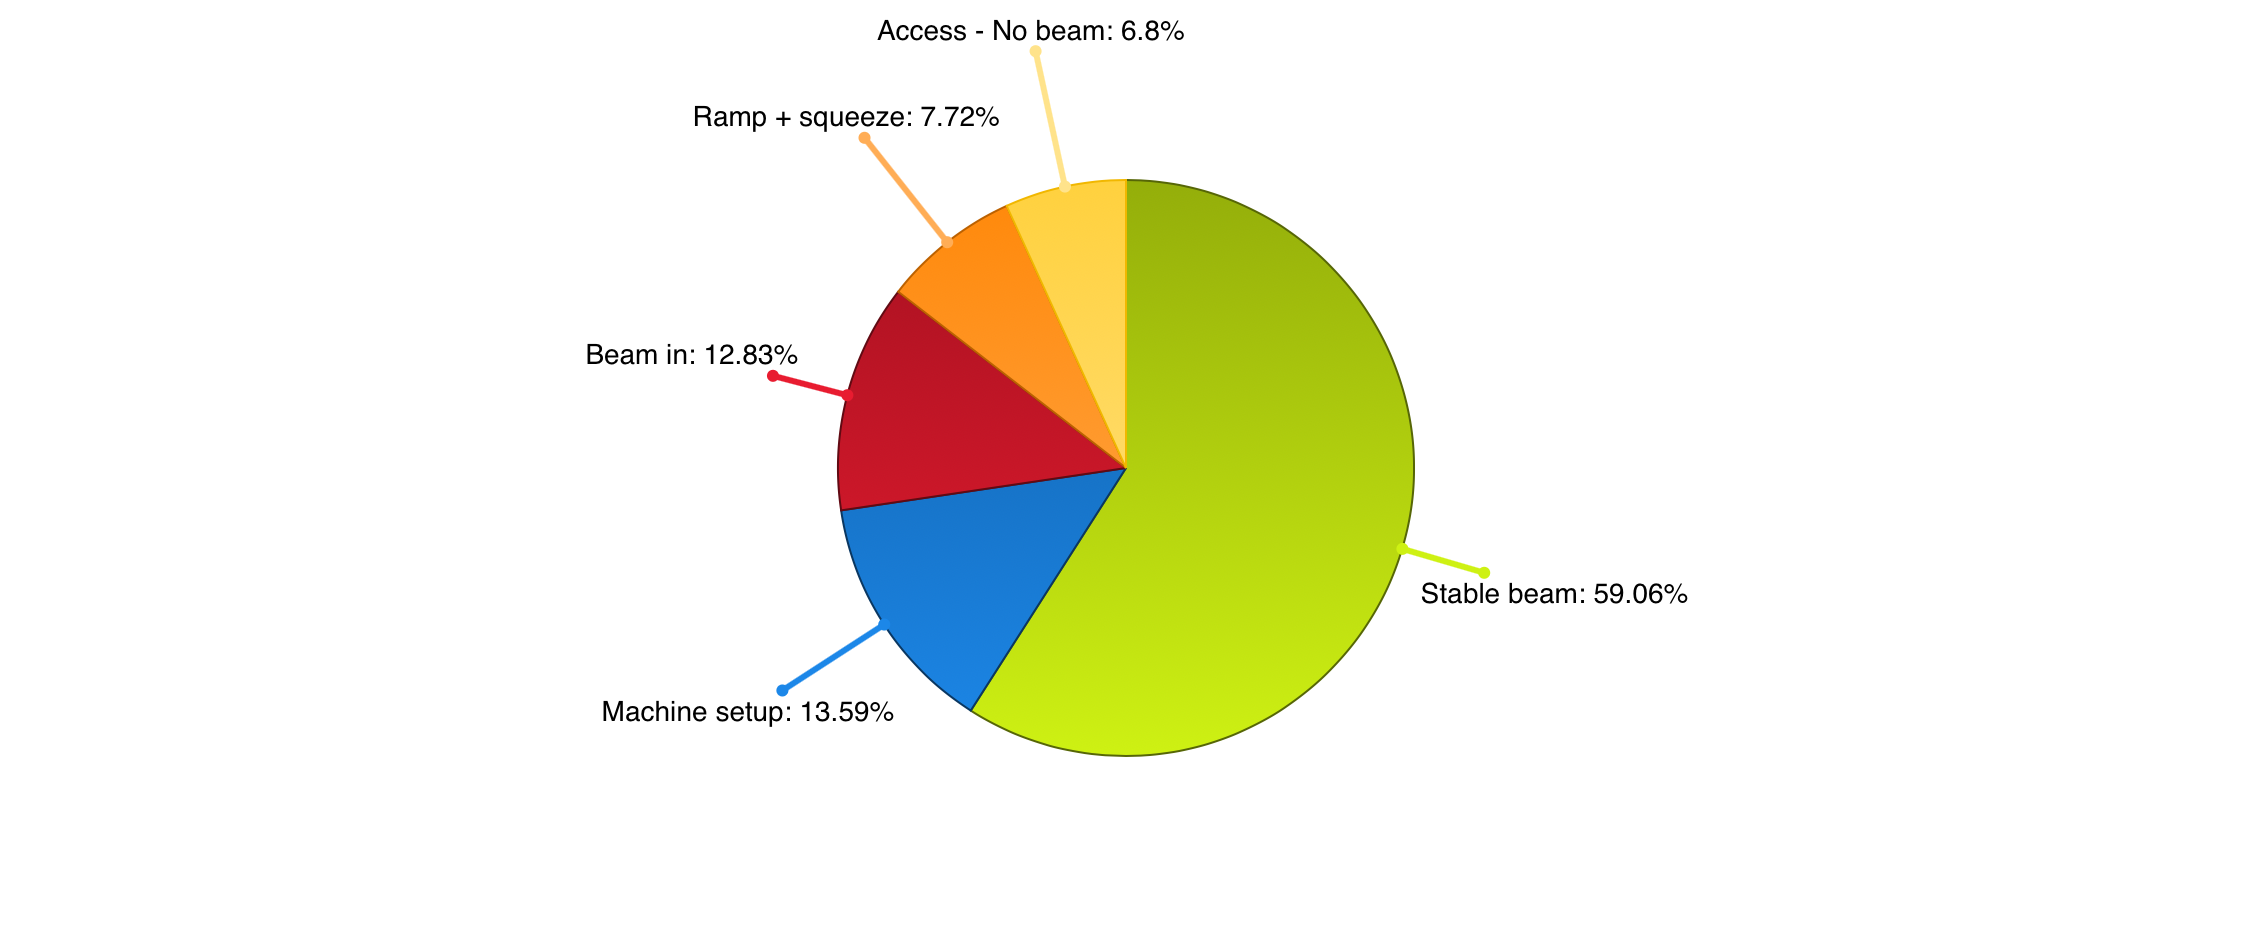
\includegraphics[width=17cm]{8TeVRunefficency}
\centering
\caption{LHC state during the 8 TeV run. }
\label{fig:RunEff}
\end{figure}

During the 8 TeV data collection period approximately 180 million minimum bias events were recorded, as summarized in table \ref{tab:RunSummary}.  These events are separated into periods, which dictate the particular beam and detector configurations during the data taking.The 8 TeV data is broken into 7 periods with approximately 181 million minimum bias events recorded.  This minimum bias sample corresponds to an integrated luminosity, $\mathscr{L}_{int}$, of $8.95 \, pb^{-1}$ during this time period\cite{ALICE-PUBLIC-2017-002}.

\begin{table}[hb]
\label{tab:RunSummary}
\begin{center}
\begin{tabular}[b]{|c|c|c|}
	\hline
	Period & \# of runs & \# of Min Bias events \\ \hline
	LHC12c & 89 & $\sim \,$24 M \\ \hline
	LHC12d & 140 & $\sim \,$62 M \\ \hline
	LHC12e & 5 & $\sim \,$2 M \\ \hline
	LHC12f & 56 & $\sim \,$15 M \\ \hline
	LHC12g & 8 & $\sim \,$0.4 M \\ \hline
	LHC12h & 159 & $\sim \,$75 M \\ \hline
	LHC12i & 40 & $\sim \,$3 M \\ \hline
	Total & 497 & $\sim \,$181 M \\ \hline

\end{tabular}
\end{center}
\caption{2012 8 TeV data taking period.}
\end{table}

Approximately, 15\% of the data sampled is unusable due to malfunctions in TPC chambers, EMCal super modules, the electronics for the EMCal or TPC, and   
\section{Raw measurements}
The ALICE experiment is capable of two types of jet reconstruction, charged and full jets.  Charged jets use information from the charged particle tracking detectors, such as the ITS and TPC, in conjunction with a jet finding algorithm to identify jets.  Full jets implement a similar procedure but also incorporates the EMCal in order to 

\subsection{Raw Jet Momentum Spectra in pp Collisions}

\subsection{Acceptance Correction}
Jet spectra, cross sections, and ratios of cross sections are reported over the full azimuth angle and psuedorapidity acceptance.  However, due to jets being constrained to the EMCal, a geometric factor is used to correct for the limited acceptance of the detector.  This thesis uses a maximum jet radius of 0.5 to help study the effects of wide angle radiation on jet fragmentation.  Heavy-ion use smaller jet radii, typically of 0.2, to help negate the high multiplicity background.  Due to these geometric corrections the centroid of a jet is constrained to,

\begin{equation}
|\eta_{jet}| \leq 0.7 - R, \; 1.4 + R \leq \phi_{jet} \leq 3.14 -R.
\label{eq:jetconstration}
\end{equation}

\begin{equation}
A(p_{T}) = \frac{(1.4 - 2R) \times (1.745 - 2R)}{2 \pi}.
\label{eq:acceptance}
\end{equation}

For jets between R = 0.1 through R = 0.5 the following jet acceptance corrections are used.

\begin{table}[hb]
\label{tab:AcceptanceFactor}
\begin{center}
\begin{tabular}[b]{|c|c|c|}
	\hline
	Jet R & $A(p_{T})$ \\ \hline
	0.1 & 0.296 \\ \hline
	0.2 & 0.214\\ \hline
	0.3 & 0.146\\ \hline
	0.4 & 0.091\\ \hline
	0.5 & 0.048\\ \hline
\end{tabular}
\end{center}
\caption{EMCal jet acceptance for radii 0.1 - 0.5.}
\end{table}








\section{Unfolding}

The reconstructed jet $p_{T}$ has a number of detector effects `folded' into the measurement.  In order to have results which can be compared to theoretical calculations or between experiments these effects must be accounted and corrected.  `Unfolding' is the method by which these results are corrected by and it accounts for a number of effects including; tracking and momentum inefficencies associated with the tracking detectors, material loss in the detector, hadronic corrections in the EMCal, and gaps in the acceptance of the detector and dead regions.  In this analysis the response matrix is constructed by propagating the truth-level particle jets generated from a MC simulation through a simulation of the detector during the time period that the data taking occurred.  

\subsection{Corrections to particle Level}

Unfolding was performed using the \verb+RooUnfold+\cite{Adye:2011gm} software package.  The response matrix was constructed by embedding the final state hadrons created from a PYTHIA generated event into a GEANT3 simulation of the ALICE detector calibrated for each of the 8 TeV periods.  Corrections are applied using the bin-by-bin\cite{Cowan:2002in} algorithm. 

\begin{equation}
C_{MC} \big( p_{T}^{low} : p_{T}^{high} \big) =  \frac{  \int^{p_{T}^{high}}_{p_{T}^{low}} dp_{T} \; \frac{dF^{uncorr}_{meas}}{dp_{T}} \times \frac{d^{2}N^{particle}_{MC}/d\eta \, dp_{T}}{d^{2}N^{detector}_{MC}/d\eta \, dp_{T}}  } { \int^{p_{T}^{high}}_{p_{T}^{low}} dp_{T} \; \frac{dF^{uncorr}_{meas}}{dp_{T}} }
\label{eq:binbybin}
\end{equation}

\noindent
where $d^{2}N^{particle}_{MC}/dp_{T} \, d\eta$ is the PYTHIA level inclusive jet spectra, $d^{2}N^{detector}_{MC}/dp_{T} \, d\eta$ is the GEANT 3 level inclusive jet spectra, $dF^{uncorr}_{meas} / dp_{T}$ is a weight function which minimizes the dependence on the two simulation spectra shapes, finally $p_{T}^{low}$ and $p_{T}^{low}$ are the lower and upper bin limits.  

\subsection{Response Matrix}
The detector response is calculated on a jet-by-jet basis.  The particle-level jet centroid ($\phi_{part}$,$\eta_{part}$)is matched to the detector-level jet via a constrain on the displaced distance between the two jet centroids in ($\phi$,$\eta$).  This distance was constrained to: $\Delta  R = \sqrt{(\phi_{part} - \phi_{det})^{2} + (\eta_{part} - \eta_{det})^{2}} \leq 0.25 \; $ for R = 0.3 to R = 0.5 jets and $\Delta R \leq 0.0 \;$ for R = 0.1 and R = 0.2 jets.  The resulting response matrices are shown in


\subsection{Unfolded Spectra}

\section{EMCal Triggered Data}

In addition with the minimum bias data collected, the EMCal was used during the 8 TeV run in order to provided an enhanced data set that is preferential to hard processes.   The Level-1 trigger\cite{Bourrion:2010js} in the EMCal has a associated trigger, $\epsilon$, of 

\begin{equation}
	\epsilon = \frac{N^{Triggered}_{events}}{N^{MinBias}_{events}} \times \frac{d^{2} N_{Triggered}^{jet}}{d\eta \, dp_{T}} \Bigg/  \frac{d^{2} N_{MinBias}^{jet}}{d\eta \, dp_{T}} 
\label{eq:xsecdef}
\end{equation}

\section{Systematic Uncertainties}

Systematic uncertainties arise due to our limited knowledge of the precise operating conditions and performance of the experiment and also due to any bias in our understanding of how to fundamental model the interactions.  They systematics may therefore be broken into two components: uncertainties to the jet energy scale (JES) which shifts the momentum spectra along the x-axis and uncertainties in the jet yield which shift the spectra along the y-axis.  The systematical and statistical uncertainties presented in this analysis will be presented as errors to the yield of the spectra.  Due to the fact that the $p_{T}$ distribution follows a power law function, $dN/dp_{T} \sim p_{T}^{-5}$ uncertainties in the JES are converted to yield uncertainties by dividing each one by 5.
Due to the low statistics at the highest $p_{T}$ bins in this analysis, uncertainties in this regime my have large statistical fluctuations.  Small ,systematic variations for the input of the jet spectra will have a dramatic effect over sparsely filled bins versus bins with a low granularity.  As such it may be necessary to extrapolate the systematic from a low $p_{T}$ bin to those at the highsest $p_{T}$ range.  The systematics were performed on both the MB and EMCal triggered data samples but no large variation was observed between the two, thus only the uncertainties from the MB sample are shown and are extrapolated to the triggered data.


\subsection{Systematic Uncertainty to Jet Energy Scale}

\subsubsection{Tracking Efficiency}
Corrections for the tracking efficiency were performed by randomly throwing out 5\% of the tracks from each event from the 8 TeV data samples and reperforming jet on the altered data.  All of the inputs for jet finding were maintained.


\begin{figure*}[t!]
$\begin{array}{rl}
    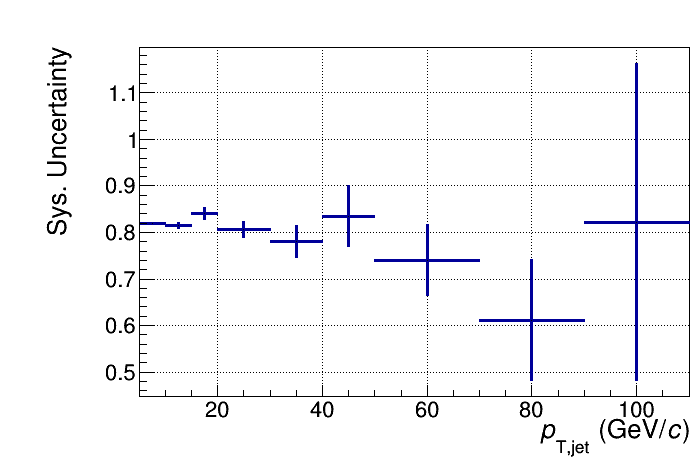
\includegraphics[width=0.5\textwidth]{SysR02_TrkEff} &
    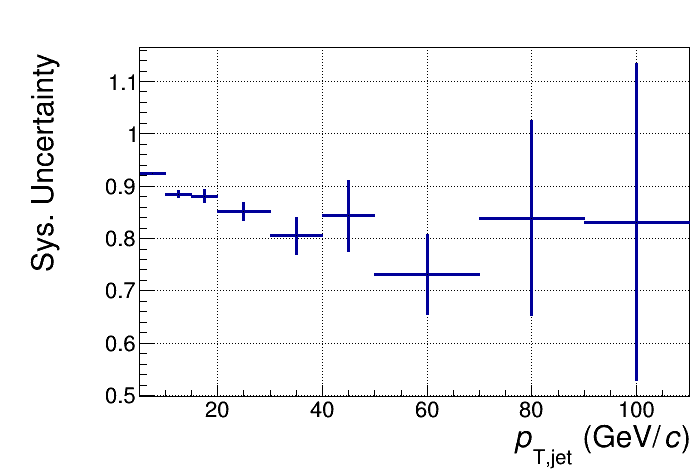
\includegraphics[width=0.5\textwidth]{SysR03_TrkEff}\\
    \multicolumn{2}{c}{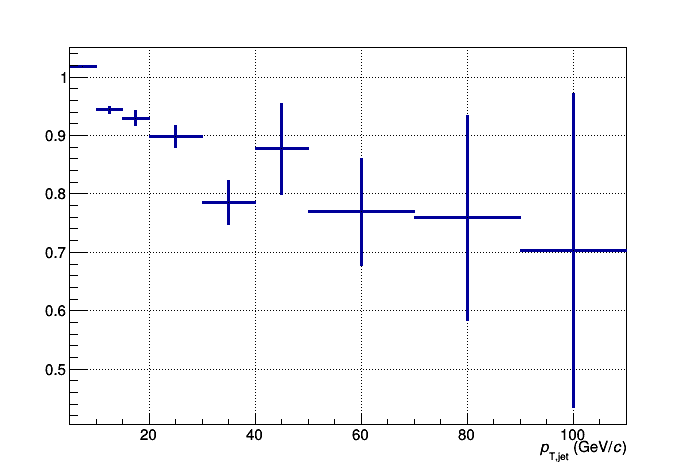
\includegraphics[width=0.5\textwidth]{SysR04_TrkEff}}
\end{array}$
\caption[Systematic due to TPC tracking efficiency.]{\label{fig:trkeff}Systematic due to TPC tracking efficiency.}
\end{figure*}

\noindent
Figure \ref{fig:trkeff}

\subsection{Systematic Uncertainty to Jet Yield}



\subsubsection{Luminosity Uncertainty}

The luminosity of a hadronic collider, $\mathscr{L}$, is given by the expression



\begin{equation}
\mathscr{L} = \frac{R}{\sigma}
\label{eq:xlumdef}
\end{equation}

The luminosity along with its uncertainty were determined during a a special Van der Meer scan run in April of 2012\cite{ALICE-PUBLIC-2017-002}.  The total systematic uncertainty for the minimum bias (MB) trigger were obtained by measuring the visible cross section using the T0 and V0 detectors.  The MB trigger was defined as V0AND which required a hit in both tjhe V0A and V0C.  The cross section was reported as being a combined average for MB with the V0AND as, 

\begin{equation}
\sigma_{V0} = (55.8 \pm 1.2) mb
\label{eq:xlumdef}
\end{equation}

with a combined systematic uncertainty of 2.19\% on the visible cross section and 2.60\% on the luminosity. 


\subsection{Total Uncertainty}

\section{Corrected pp jet cross section}


\subsection{Comparisons to pQCD predictions}

\subsection{Jet Cross Sections and Ratios}



